\documentclass[../Article_Model_Parameters.tex]{subfiles}
\graphicspath{{\subfix{../Figures/}}}
\begin{document}
	
	\label{CH: Results}
	
	The sensitivity equations were solved simultaneously with the original process model. The focus of this work is to investigate the influence of inlet temperature, pressure and mass flow-rate on the state-space as wall as on the extraction yield. 
	
	The increase of the mass-flow rate affects the whole system simultaneously in the spatial direction. The change in mass flow-rate makes the fluid moves faster, but its thermodynamic state is not affected. As the result, the  Figure \ref{fig:Sensitivty_F_P} show no change in pressure during the simulation. 
    
    \begin{figure}[h!]
    	\centering
    	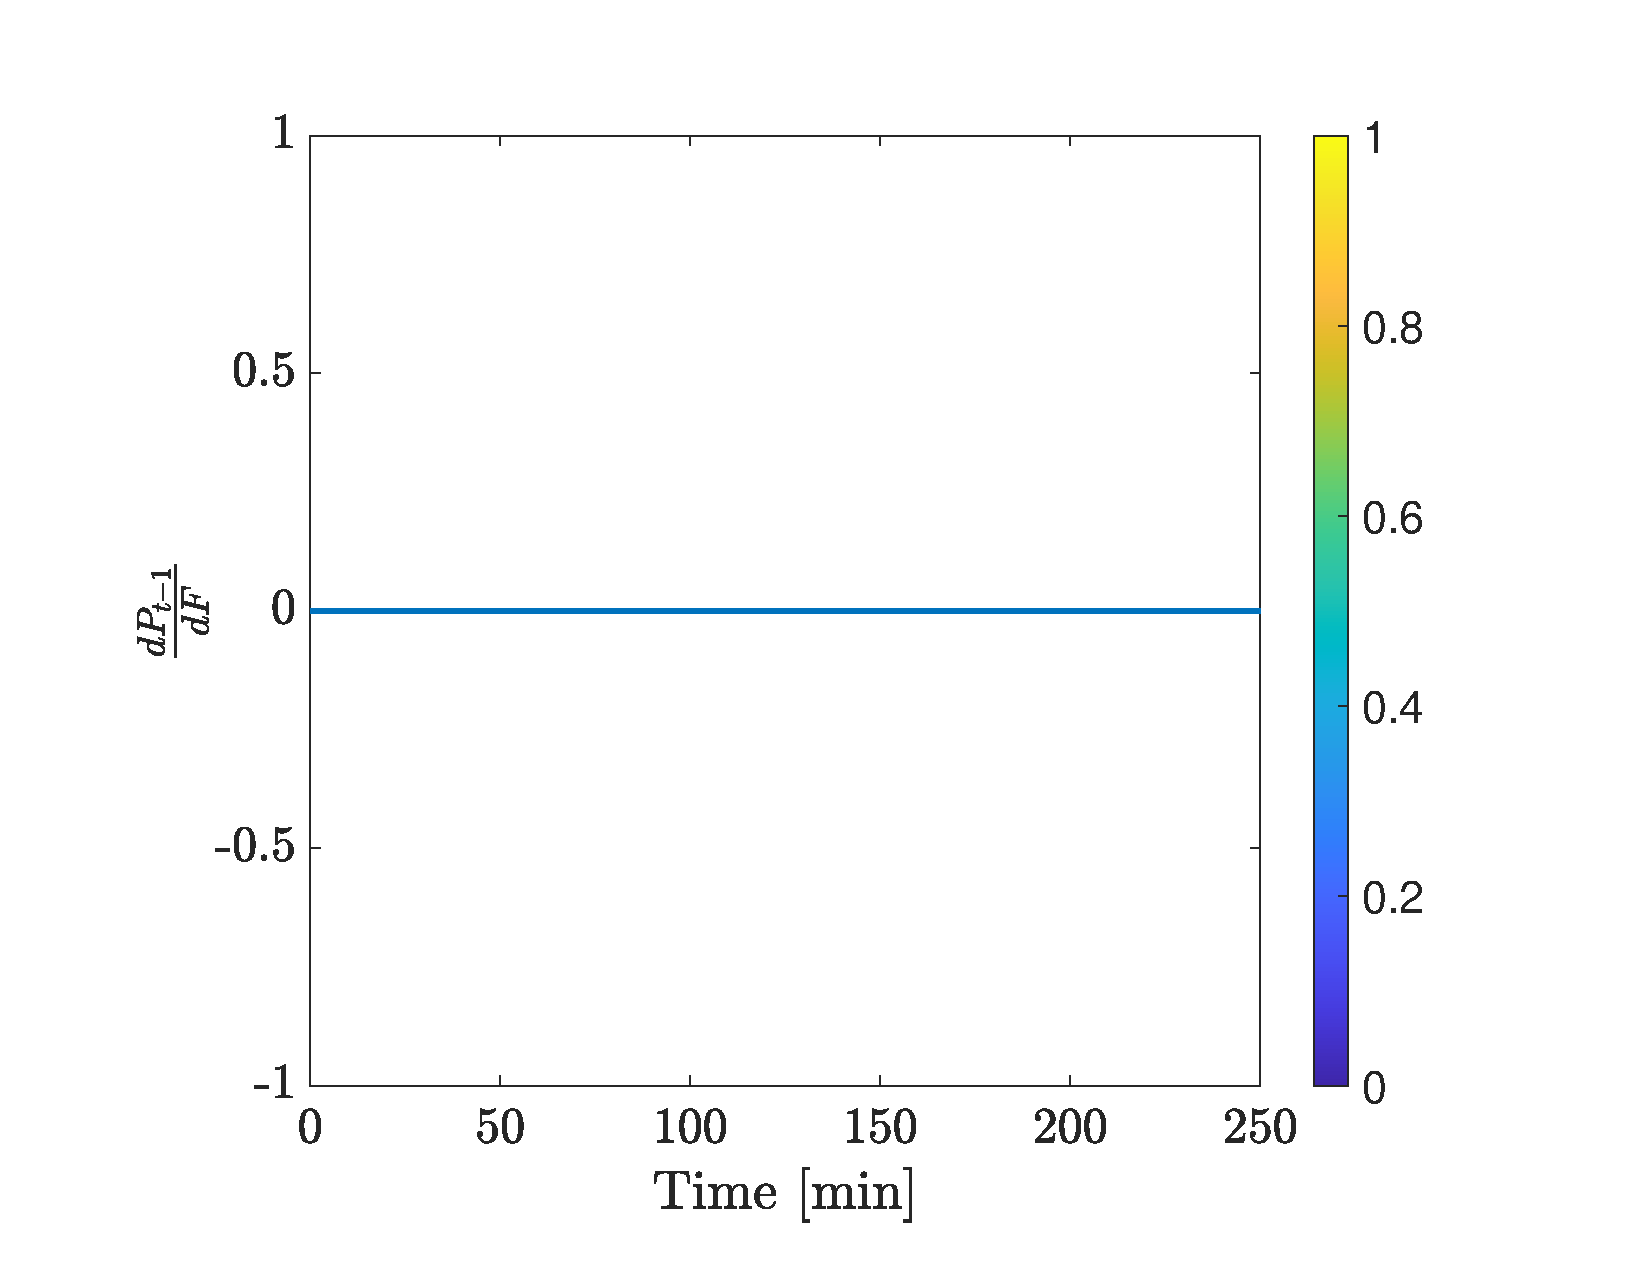
\includegraphics[trim = 3cm 0cm 0cm 0cm,clip,width=\columnwidth]{/Results_sensitivity/P_F.pdf}
    	\caption{The effect of $F$ change on $P$}
    	\label{fig:Sensitivty_F_P}
    \end{figure}
    
    Similarly, the energy in the system (defined as $\rho \times h$) is not affected as presented on Figure \ref{fig:Sensitivty_F_H}.
    
    \begin{figure}[h!]
    	\centering
    	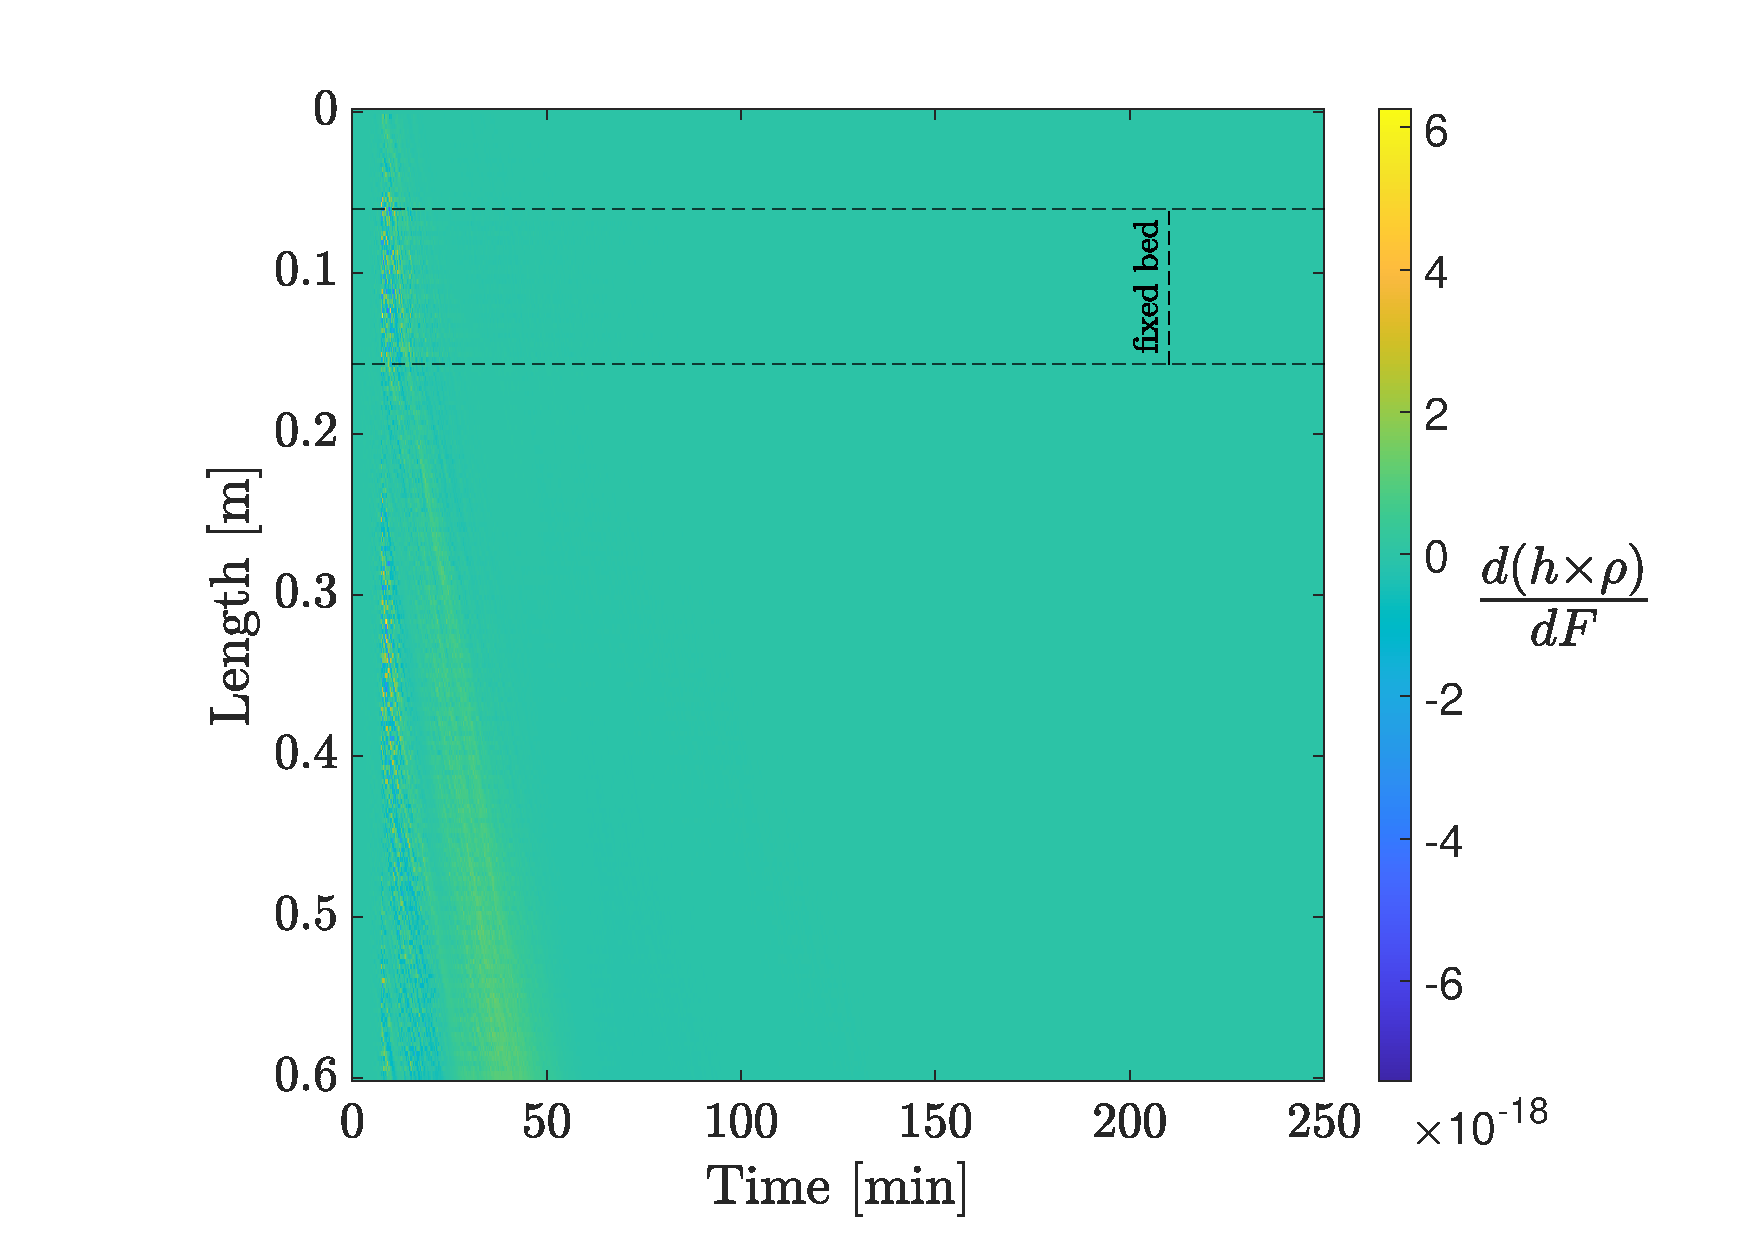
\includegraphics[trim = 3cm 0cm 0cm 0cm,clip,width=\columnwidth]{/Results_sensitivity/H_F.pdf}
    	\caption{The effect of $F$ change on $\rho \times h$}
    	\label{fig:Sensitivty_F_H}
    \end{figure}
    
    The increase in the mass flow-rate affects the concentration gradient and accelerate the extraction kinetic. The acceleration 
    
    \begin{figure}[h!]
    	\centering
    	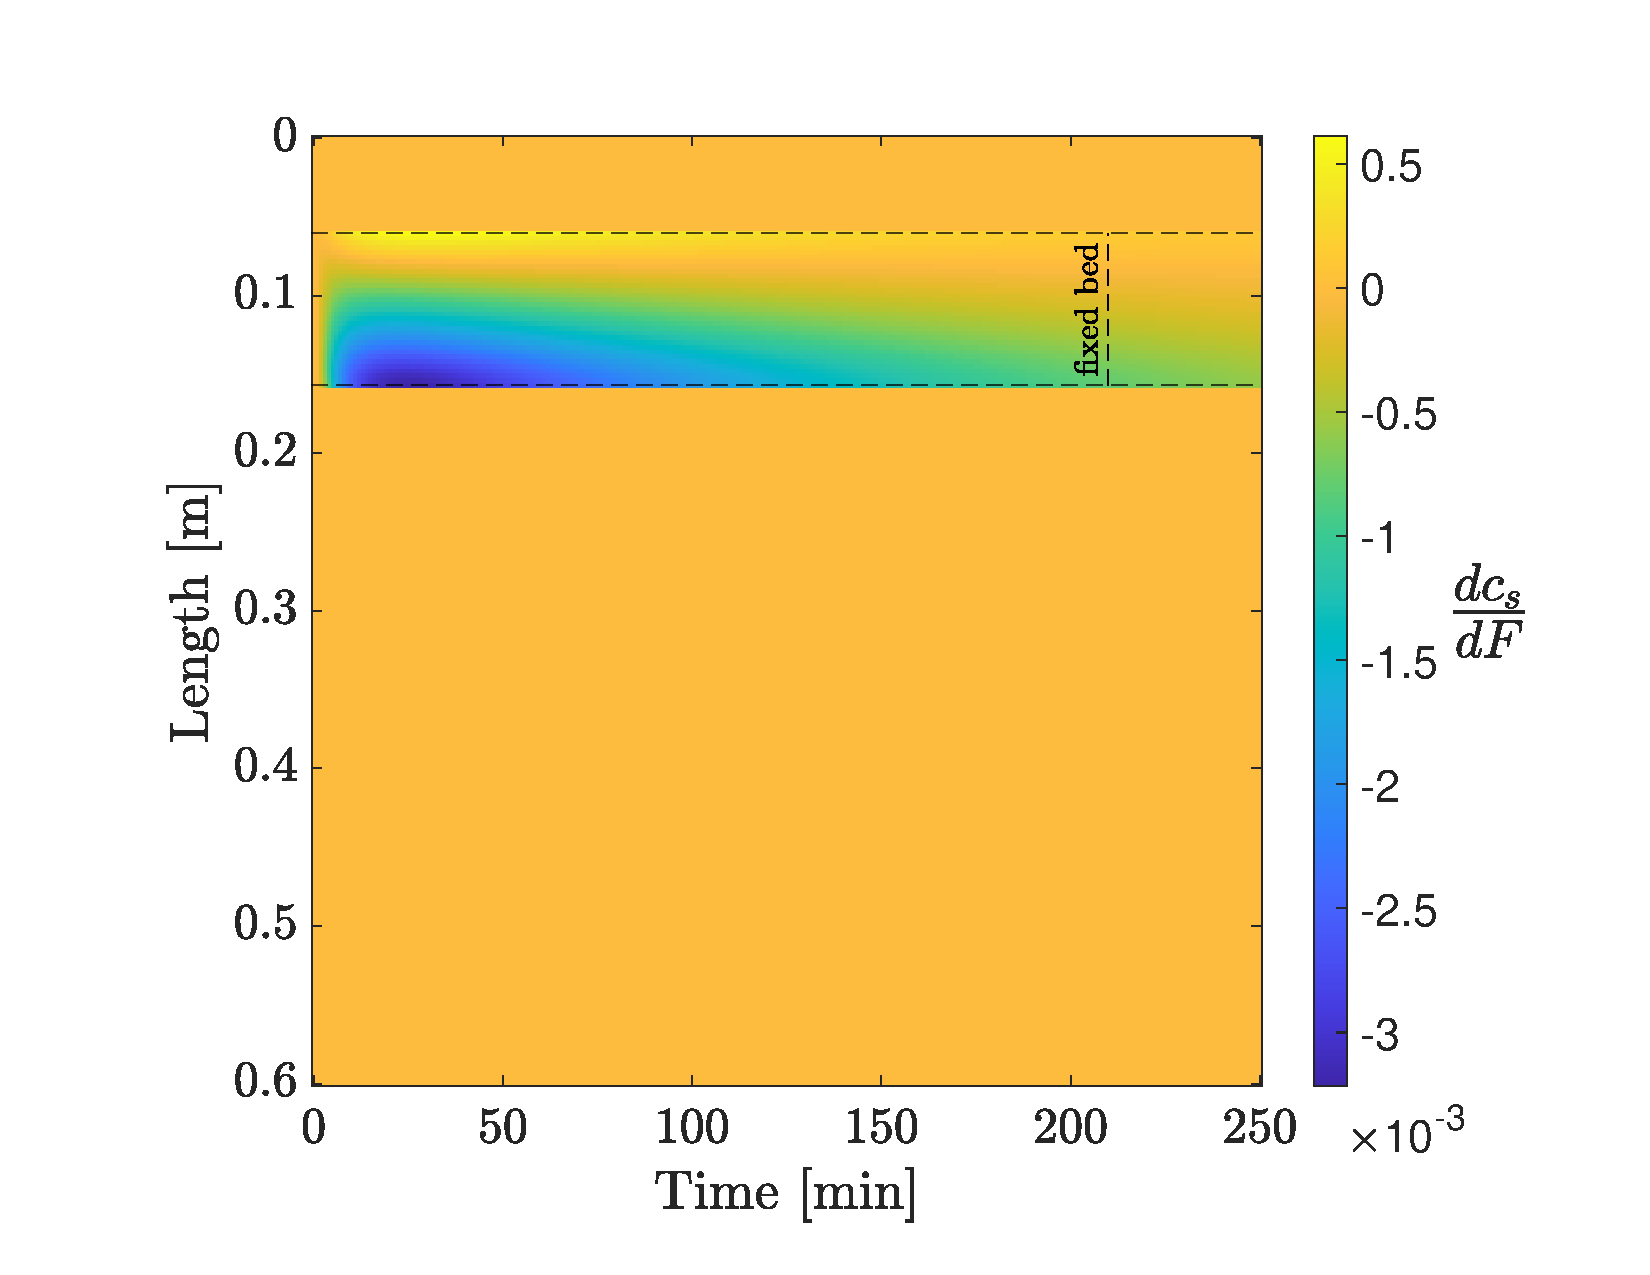
\includegraphics[trim = 3cm 0cm 0cm 0cm,clip,width=\columnwidth]{/Results_sensitivity/CS_F.pdf}
    	\caption{The effect of $F$ change on $C_s$}
    	\label{fig:Sensitivty_F_CS}
    \end{figure}
    
    \begin{figure}[h!]
    	\centering
    	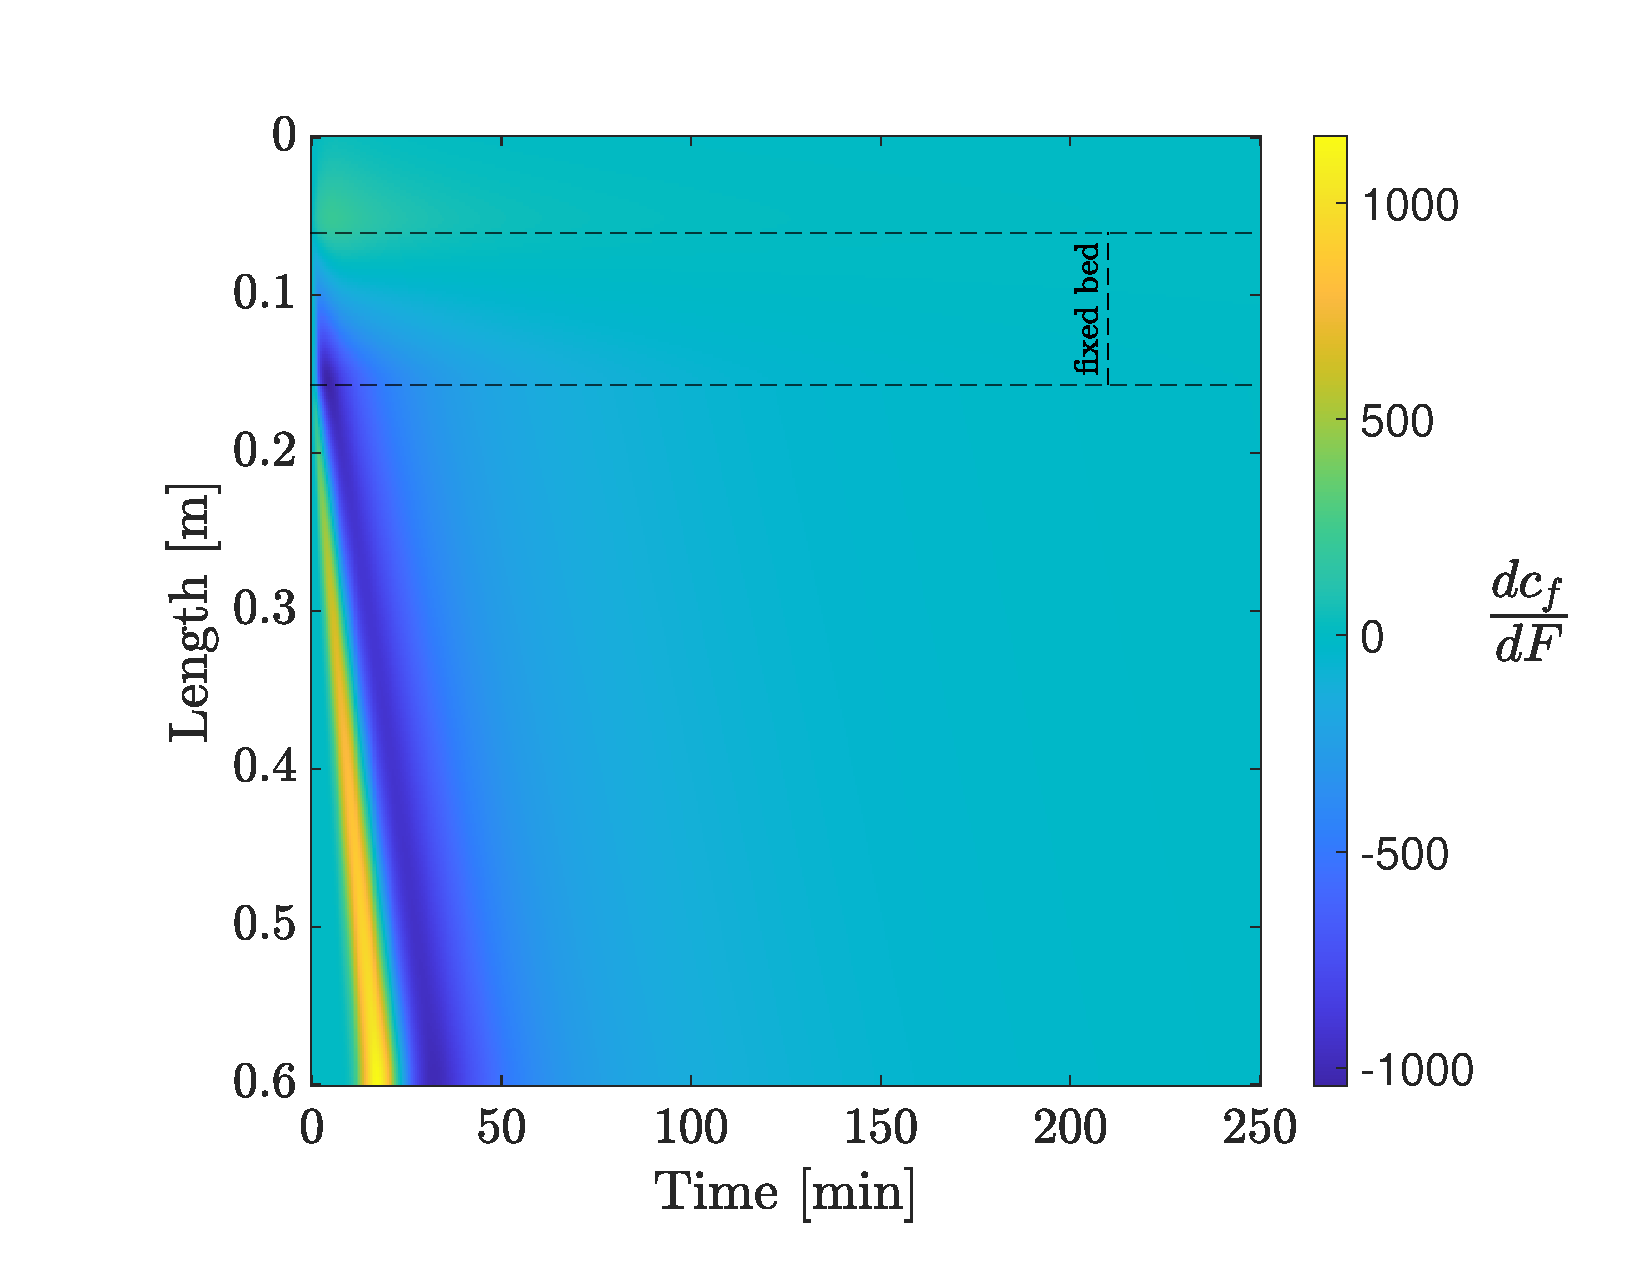
\includegraphics[trim = 3cm 0cm 0cm 0cm,clip,width=\columnwidth]{/Results_sensitivity/CF_F.pdf}
    	\caption{The effect of $F$ change on $C_f$}
    	\label{fig:Sensitivty_F_CF}
    \end{figure}
    
	
\end{document}